\documentclass[11pt,a4paper]{article}
\usepackage[T1]{fontenc}
\usepackage[left=2cm, right=2cm, top=2cm, bottom=2cm]{geometry}
\usepackage{graphicx}
\usepackage{mathtools}
\usepackage{amssymb}
\usepackage{amsthm}
\usepackage{thmtools}
\usepackage{xcolor}
\usepackage{nameref}
\usepackage[colorlinks=true, linkcolor=blue, citecolor=cyan]{hyperref}
\usepackage{natbib} 
\usepackage{tkz-graph}


\newcommand{\grad}{\operatorname{grad}}
\newcommand{\curl}{\operatorname{curl}}
\renewcommand{\div}{\operatorname{div}}
\newcommand{\img}{\operatorname{img}}
\renewcommand{\span}{\operatorname{span}}


\title{Some Resolved Confusions on Graph Homology and Cohomology}
\author{Ali Fele Paranj}



\begin{document}
	
	\maketitle
	\begin{abstract}
		In this document I will review the topics of the homology and cohomology of graphs. I will not be using the most exact language in this note and my main aim is to highlight some of the most common mistakes and confusions that one might face when reading about this topic (at least to talk about the ones that occurred to me.)
		
	\end{abstract}
	
	
	Most of my exploration in this area starting with the graph shown below and all sort of questions it led to.
	\begin{figure}[h!]
		\centering
		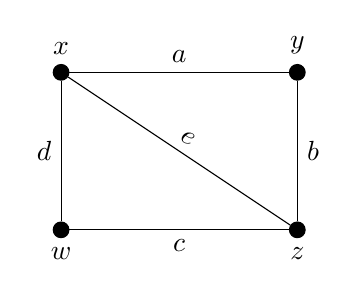
\begin{tikzpicture}
			% Nodes
			\node[draw, circle, fill=black, inner sep=2pt, label=above:$x$] (x) at (0,2) {};
			\node[draw, circle, fill=black, inner sep=2pt, label=above:$y$] (y) at (3,2) {};
			\node[draw, circle, fill=black, inner sep=2pt, label=below:$w$] (w) at (0,0) {};
			\node[draw, circle, fill=black, inner sep=2pt, label=below:$z$] (z) at (3,0) {};
			
			% Edges
			\draw (x) -- (y) node[midway, above] {$a$};
			\draw (y) -- (z) node[midway, right] {$b$};
			\draw (z) -- (w) node[midway, below] {$c$};
			\draw (w) -- (x) node[midway, left] {$d$};
			\draw (x) -- (z) node[midway, sloped, above] {$e$};
		\end{tikzpicture}
	\end{figure}
	
	As a part of my master's thesis project, I had to study different algebraic structures of graphs. So I explored these structures as discussed in \cite{Gross2005}. Somewhere in chapter 4 of this book (where you can also see the graph above), we read that the dimension of the cycle space (the elements in the edge space, that has zero boundary, i.e. $ Mx = 0 $, where $ M $ is the incidence matrix) is called the betti number. So, considering $ \{a,e,c\}  $ as an spanning tree of the graph above, then the basis cycles of the graph above will be the cycles
	\[ \{ a,b,e \}, \ \{e,c,d\}. \]
	So this space as dimension 2, hence the betti $ \beta_2 $ number of this graph is $ 2 $ (this results is in the chapter four of \cite{Gross2005}).
	
	On the other hand, by following the definition of $ \beta_2 $, that is the rank of the $ n^\text{th} $ homology group, we find different answers. I constructed a chain complex for this graph according to \cite{Lim2019} as follows
	\[ W_V \xleftarrow{\div} W_E \xleftarrow{\curl^*} W_T,  \tag{1} \]
	where the boundary operators are given as
	\[ \div = \begin{pmatrix}
		1 & 0 & 0 & 1 & 1 \\
		1 & 1 & 0 & 0 & 0 \\
		0 & 1 & 1 & 0 & 1 \\
		0 & 0 & 1 & 1 & 0
	\end{pmatrix}, \qquad
	\curl^* = \begin{pmatrix}
		1 & 0 \\
		1 & 0 \\
		0 & 1 \\
		0 & 1 \\
		1 & 1 
	\end{pmatrix} \]
	Then by definition the 1st homology group is the quotient space
	\[ H^1 = \frac{\ker \div }{\img \curl^*}. \]
	In words, this is the space of cycles module boundaries. We do a simple calculation to find the dimension of the kernel of this matrix (mod 2) (observe that since the vector spaces $ W_V, W_E $ and $ W_T $ are defined over field $ F_2 $ (see \cite{Gross2005} chapter 4), we do the operations in mod 2). We can do a mod 2 row reduction operations to get the reduced matrix
	\[ \begin{pmatrix}
		1 & 0 & 0 & 1 & 1 \\
		0 & 1 & 0 & 1 & 1 \\
		0 & 0 & 1 & 1 & 0 \\
		0 & 0 & 0 & 0 & 0
	\end{pmatrix}. \]
	This matrix has rank 3, so the nullity will be $ 5 - 3 = 2 $. Let $ X = (x_1,x_2,x_3,x_4,x_5)^T $. From the reduced system we will have
	\[ x_1 + x_4 + x_5 = 0, \quad x_2 + x_4 + x_5 = 0, \quad x_3 + x_4 = 0. \]
	By solving for the free variables we will get 
	\[
	\ker \div = \operatorname{span} \left\{
	\begin{pmatrix}
		1 \\ 1 \\ 0 \\ 0 \\ 1
	\end{pmatrix},
	\begin{pmatrix}
		0 \\ 0 \\ 1 \\ 1 \\ 1
	\end{pmatrix}
	\right\}.
	\]
	
	This is precisely that column space of $ \curl^* $. This reveals that $ H^1 = \{0\} $ is a trivial group, hence its rank is zero, thus $ \beta_1 = 0 $. This is an apparent contradiction to what we had above, where we calculated that $ \beta_1 = 2 $.
	
	Trying to resolve the paradox, I constructed a co-chain complex as below (the reason was that I thought maybe the betti number is the rank of the $ k^\text{th} $ \emph{cohomology} group rather than the rank of the $ k^\text{th} $ \emph{homology} group.)
	\[ W_V \xrightarrow{\grad} W_E \xrightarrow{\curl} W_T, \tag{2}\]
	where the $ \grad $ and $ \curl $ operators are given as
	\[ \grad = \begin{pmatrix}
		1 & 1 & 0 & 0 \\
		0 & 1 & 1 & 0 \\
		0 & 0 & 1 & 1 \\
		1 & 0 & 0 & 1 \\ 
		1 & 0 & 1 & 0
	\end{pmatrix}, \qquad
	\curl = \begin{pmatrix}
		1 & 1 & 0 & 0 & 1 \\
		0 & 0 & 1 & 1 & 1
	\end{pmatrix} \]
	First, we find the dimension of the kernel of the $ \curl $ operator. To do this, first observe that $ \curl $ is already in the row reduced form. So its nullity is $ 5 -  2 = 3 $. With simple calculation it turns out that
	\[ \ker \curl =
	\ker(A) = \operatorname{span} \left\{
	\begin{pmatrix}
		1 \\ 1 \\ 0 \\ 0 \\ 0
	\end{pmatrix},
	\begin{pmatrix}
		0 \\ 0 \\ 1 \\ 1 \\ 0
	\end{pmatrix},
	\begin{pmatrix}
		1 \\ 0 \\ 1 \\ 0 \\ 1
	\end{pmatrix}
	\right\}.
	\].
	Inspecting the column space of $ \grad $ it reveals that $ \ker \curl = \img \grad $ as the first and the second vectors of the basis of $ \ker \curl $ is precisely the second and the forth columns of $ \grad $ vector and the third basis vector is the sum of the first and the last column of $ \grad $. Furthermore, observe that $ \grad $ has rank 3 as the third column is the sum of the all other columns. So the rank of the 1st cohomology group is also zero (which also agrees with what we see in \cite{Lim2019} but is in contradiction with the fact that $ \beta_1 = 2 $ as in \cite{Gross2005}).
	
	
	Then I thought all these are happening since I am working with mod 2 systems for the undirected and unweighted graphs (as $ W_V, W_E $, and $ W_T $ are built on $ \mathbb{F}_2 $). The ``topological caveats'' discussed in section 5.1 of \cite{Lim2019} made this thought more strong. But then I noticed that in the calculations above, I am not using any of the tools that \cite{Lim2019} is developing during section 1 and section 2 of that article, and all of my calculations above are the bare-metal calculations, and there is no possible way that the ``topological caveats'' might be the reason for this paradox.
	
	These paradoxical observations come to an end when I read \cite{dewan2016graph}, where in section 6 of this article, the authors mentions the following chain complex (that is also called the ordinary homology of graph):
	\[ \cdots \xleftarrow{d_{-1}=0} 0 \xleftarrow{d_{0}=0} W_V \xleftarrow{d_{1}=\div} W_E \xleftarrow{d_{2}=0} 0 \xleftarrow{d_{3}=0} \cdots, \tag{3} \]
	where they assume that the spaces after $ W_E $ are trivial spaces, i.e. $ \{0\} $. With this definition of the chain complex, all of the paradoxes go away, as in this case the image of $ d_2 $ operator is the trivial subspace $ 0 $. After this observation I came across \cite{Wiki2024}, where in the section ``Higher dimensional homologies'', they also report a similar observation as mine above.
	
	In conclusion, the interpretation of the betti numbers really depends on the chain, or cochain complex of under study, i.e. it is crucial to know the all chains or co-chains in the complex and this will affect the final result. In the most simple cases we use simple chain complex (as in (3)), but for some applications (like Hodge decomposition for which see \cite{2024,Lim2019,strang2020applications} for a very good starting point to study this) we use chain complexes that are richer	(like (1),(2) above). Notice that in $ (1),(2) $ above, we have not written down that higher or lower chains when they are zero and the boundary and co-boundary operators are the trivial operators.  
	
	
	
	
	
	
	\bibliographystyle{dinat}
	\bibliography{references}
	
	
\end{document}